\section{Actividad 1: Condiciónes $I_G$ e $I_H$.}

\subsection{Actividad de Laboratorio}

\begin{itemize}
    \item 3 Multimetros
    \item SCR TIC106M
    \item Resistores de 3300$\Omega$ y dos de 4700$\Omega$
    \item Potenciómetro de 5000$\Omega$
    \item 2 Fuentes de alimentación
\end{itemize}

\paragraph{Procedimiento}
Para esta actividad se implementó el siguiente circuito:

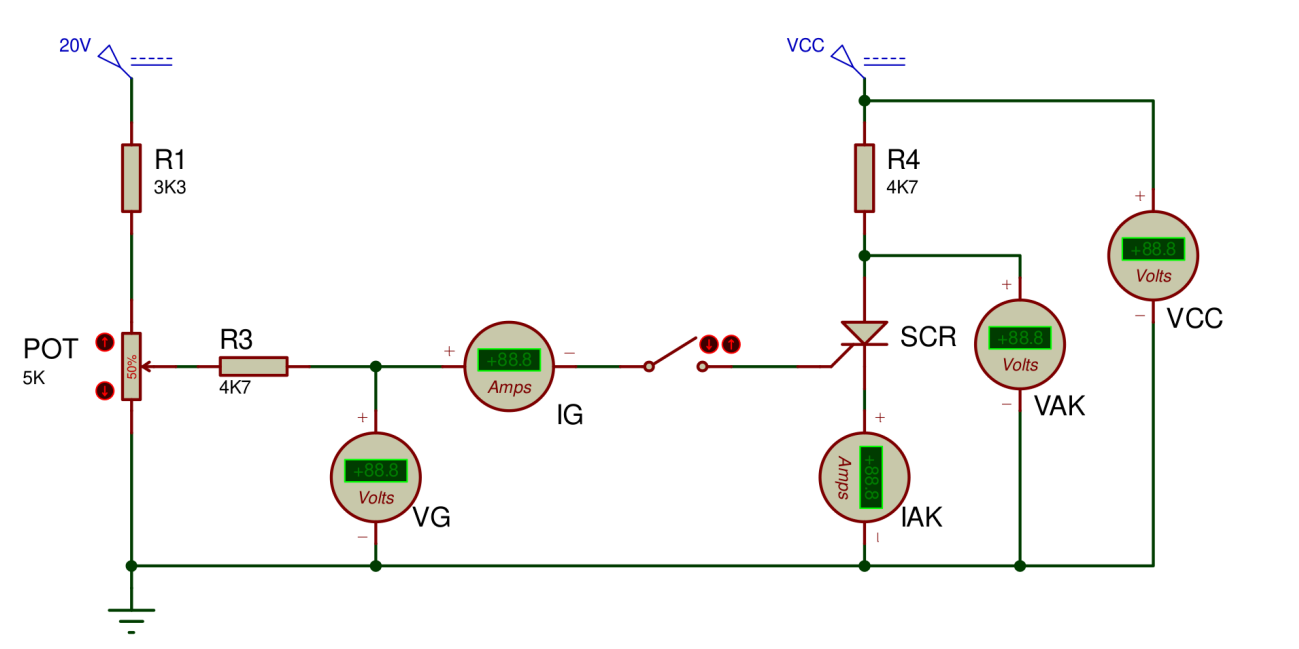
\includegraphics[width=8.08cm]{./imagenes/Circ1.png}

Primero se dejó la fuente $V_{CC}$ en 0, se cerró el interruptor y se empezó a variar el potenciometro para obtener valores de $V_G$ e $I_G$.

Luego se colocó $V_G$ en 0 y se cerró el interruptor y se colocó $V_{CC}$ en 100V. Lentamente aumentamos el valor $V_G$ hasta ver un cambio en $I_{AK}$.

Dejamos el potenciometro en el valor que nos dió el disparo y abrimos el interruptor, observando que sucede con $I_{AK}$.

Ahora manteniendo la llave abierta, bajamos $V_{CC}$ en pasos de 10V, y los ultimos 10V en pasos de 1V. Luego volver a aumentar $V_{CC}$ hasta 100V.

Cerramos el interruptor y comprobamos que los valores de $V_G$ e $I_G$ son los mismos que al principio.

Abrimos el interruptor y analizamos que sucede con $I_{AK}$.

Desconectamos las tensiones de alimentación sin mover nada y luego las volvemos a conectar, cerramos el interruptor y analizamos el comportamiento de $I_{AK}$.


\paragraph{Analisis de Resultados}

\begin{enumerate}
    \item Analizar y mencionar la alternativa que se presentó para disparar un SCR. ¿Cómo la puede explicar?. Existe otra manera de disparar el SCR sin corriente en la compuerta ¿Cual es ese método?
    \item Analizar y sacar conclusiones de las conexiones y mediciones realizadas.
\end{enumerate}


\subsection{Simulación}

Para la simulación del circuito utilizamos el siguiente esquema:

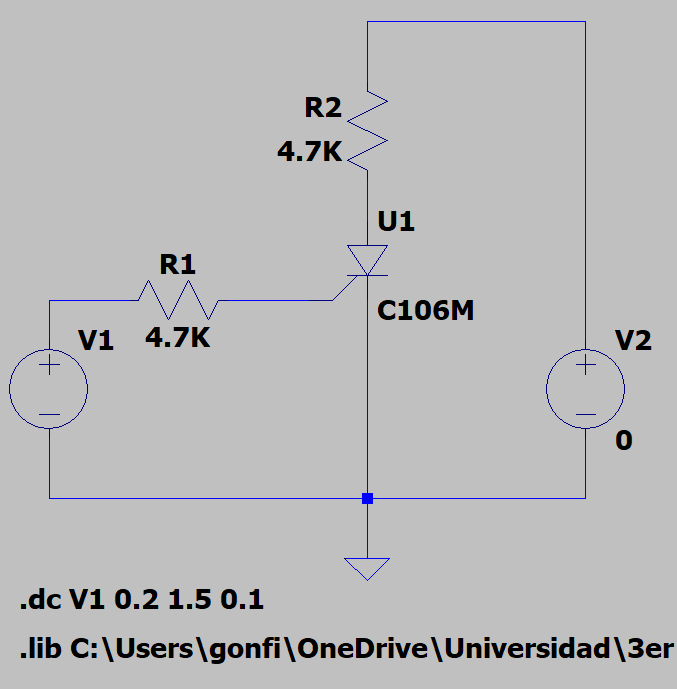
\includegraphics[width=7cm]{./imagenes/Sim1.png}

Primero establecemos la fuente $V_2$ en 0V y variamos la fuente $V_1$ de 0.2V a 1.5V en pasos de 0.1V, obteniendo la siguiente gráfica:

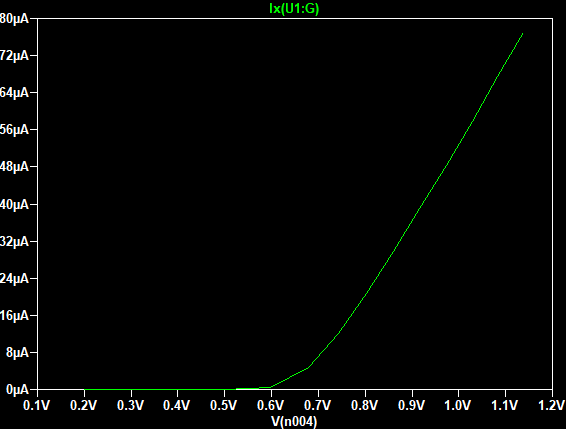
\includegraphics[width=8cm]{./imagenes/Simres1.png}

Ahora Analizaremos el disparo, para ello variaremos la fuente $V_2$ de 0V a 800V en pasos de 10V, obteniendo la siguiente gráfica:

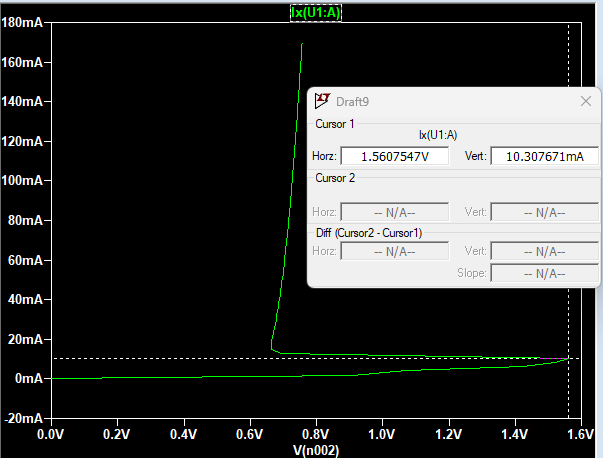
\includegraphics[width=8cm]{./imagenes/Simres2.png}

Por ultimo realizaremos un disparo controlado, dejaremos la fuente $V_2$ en 100V y variaremos la fuente $V_1$ hasta encontrar un punto donde $I_A$ cambie bruscamente, obteniendo la siguiente gráfica:

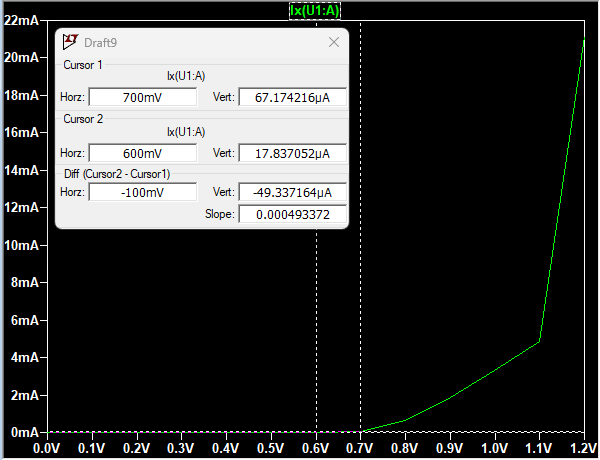
\includegraphics[width=8cm]{./imagenes/Simres3.png}

En la primera simulacion observamos que la curva tiene un comportamiento similar al de un diodo, con una caida de tension directa de aproximadamente 0.7V. En la segunda simulacion observamos que el SCR se dispara alrededor de los 1.56V. En la tercera simulacion con $V_2$ en 100V, el SCR empieza a conducir entre los 0.6V y los 0.7V como se observa en la grafica.